\def\verantwortlicher{Siegfried Zötzsche} % Dokumentverantwortlicher in Kopfzeile
\thispagestyle{empty} 

%%% Titelseite A
\vspace*{2\baselineskip}

\begin{center}
\sffamily
Universität Leipzig\\
Softwaretechnik-Praktikum\\
Sommersemester 2014
\vskip3\baselineskip

\bgroup
\Huge\textbf{Entwurfsbeschreibung\\ Vorprojekt}
\egroup
\vskip3\baselineskip

\begin{tabular}{ll}
Projekt & Graphical SPARQL Builder \\
Gruppe & s14.swp.gsb \\
Verantwortlich & \verantwortlicher\\
Erstellt am & \today \\
\end{tabular}
\end{center}

\vfill

\tableofcontents
%%% Titelseite E

\pagebreak

%%%%%%%%%%%%%%%%%%%%%%%%%%%%%%%%%%%%%%%%
\section{Allgemeines}

Um Anfragen mit SPARQL an RDF-basierte Datenbanken formulieren zu
können muss zunächst eine gewisse Einstiegshürde überwunden werden.
Selbst für weniger komplexe Anfragen müssen grundlegende Syntax und
Vokabular der SPARQL vertraut sein.

Mit dem Graphical SPARQL Builder (GSB) soll diese Einstiegshürde gesenkt
werden.
Dazu setzt der GSB auf eine graphische Repräsentation der Anfrage
gegenüber einer rein textbasierten Anfrage in SPARQL.

Zum einen soll eine Anfrage möglichst intuitiv erstellt werden können,
zum anderen soll die Anfrage auch mit minimaler Vorkenntnis von RDF
und SPARQL lesbar sein.

\section{Produktübersicht}

Abbildung~\ref{fig01} gibt eine Übersicht über die Eingliederung und Nutzung des Graphical SPARQL Builder beim Einsatz des Tools im Zusammenspiel mit beteiligten Personen und externen Softwarekomponenten:

%\begin{figure}[tbp]%
%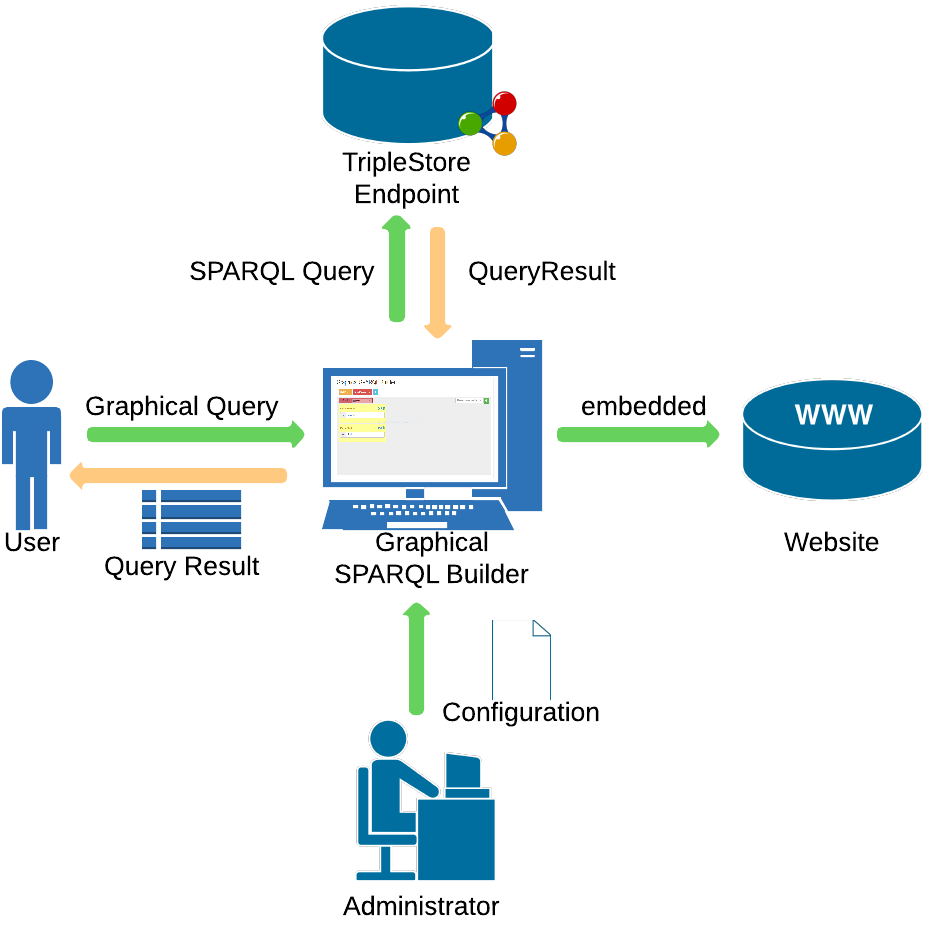
\includegraphics[width=.7\hsize]{Produktuebersicht2.png}
%\caption{Beziehung des GSB zu Anwender, Datenbank und Administration.}
%\label{fig01}
%\end{figure}
\begin{SCfigure}[20][htbp]%
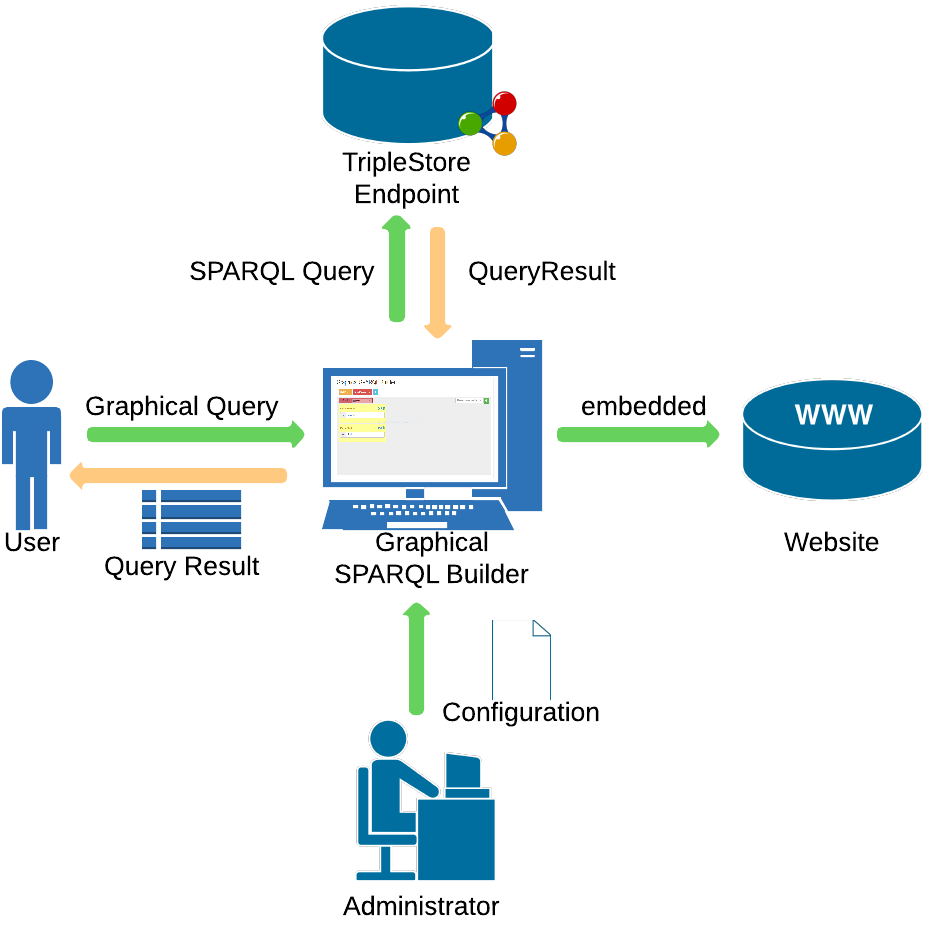
\includegraphics[width=.7\hsize]{Produktuebersicht2.png}
\caption{Beziehung des GSB zu Anwender, Datenbank und Administration.}
\label{fig01}
\end{SCfigure}

Im typischen Anwendungsfall möchte ein User (ohne SPARQL Kenntnisse)
eine Anfrage an eine RDF-basierte Datenbank stellen. 
Dazu stellt er sich die Anfrage grafisch im GSB zusammen und sendet
sie ab. Der GSB übersetzt die grafische Repräsentation der Anfrage
(zunächst in ein intern vordefiniertes JSON-Format und dann) in eine
semantisch und syntaktisch korrekte SPARQL-Anfrage. 
Das Tool sendet diese dann an einen vom Administrator eingestellten
SPARQL-Endpunkt eines TripleStores, von welchem das Anfrageergebnis
zurückgegeben wird. Der GSB leitet das Ergebnis an den User weiter.

Der Administrator hat die Möglichkeit über Konfigurationsdateien
diverse Einstellungen, wie Sprachwahl, Einschränkungen der
bereitgestellten Datenbank, Expertenansicht und zahlreiche
GUI-Anpassungen vorzunehmen.
Als Single-Page-Anwendung kann der GSB in bestehende Websites eingebettet werden.


\section{Grundsätzliche Struktur- und Entwurfsprinzipien}

Die Grundsätzliche Struktur des GSB ist im Komponentendiagramm
(s.~Abb.~\ref{fig02}) schematisch dargestellt.

%\begin{SCfigure}[20][htbp]%
\begin{figure}[tbp]%
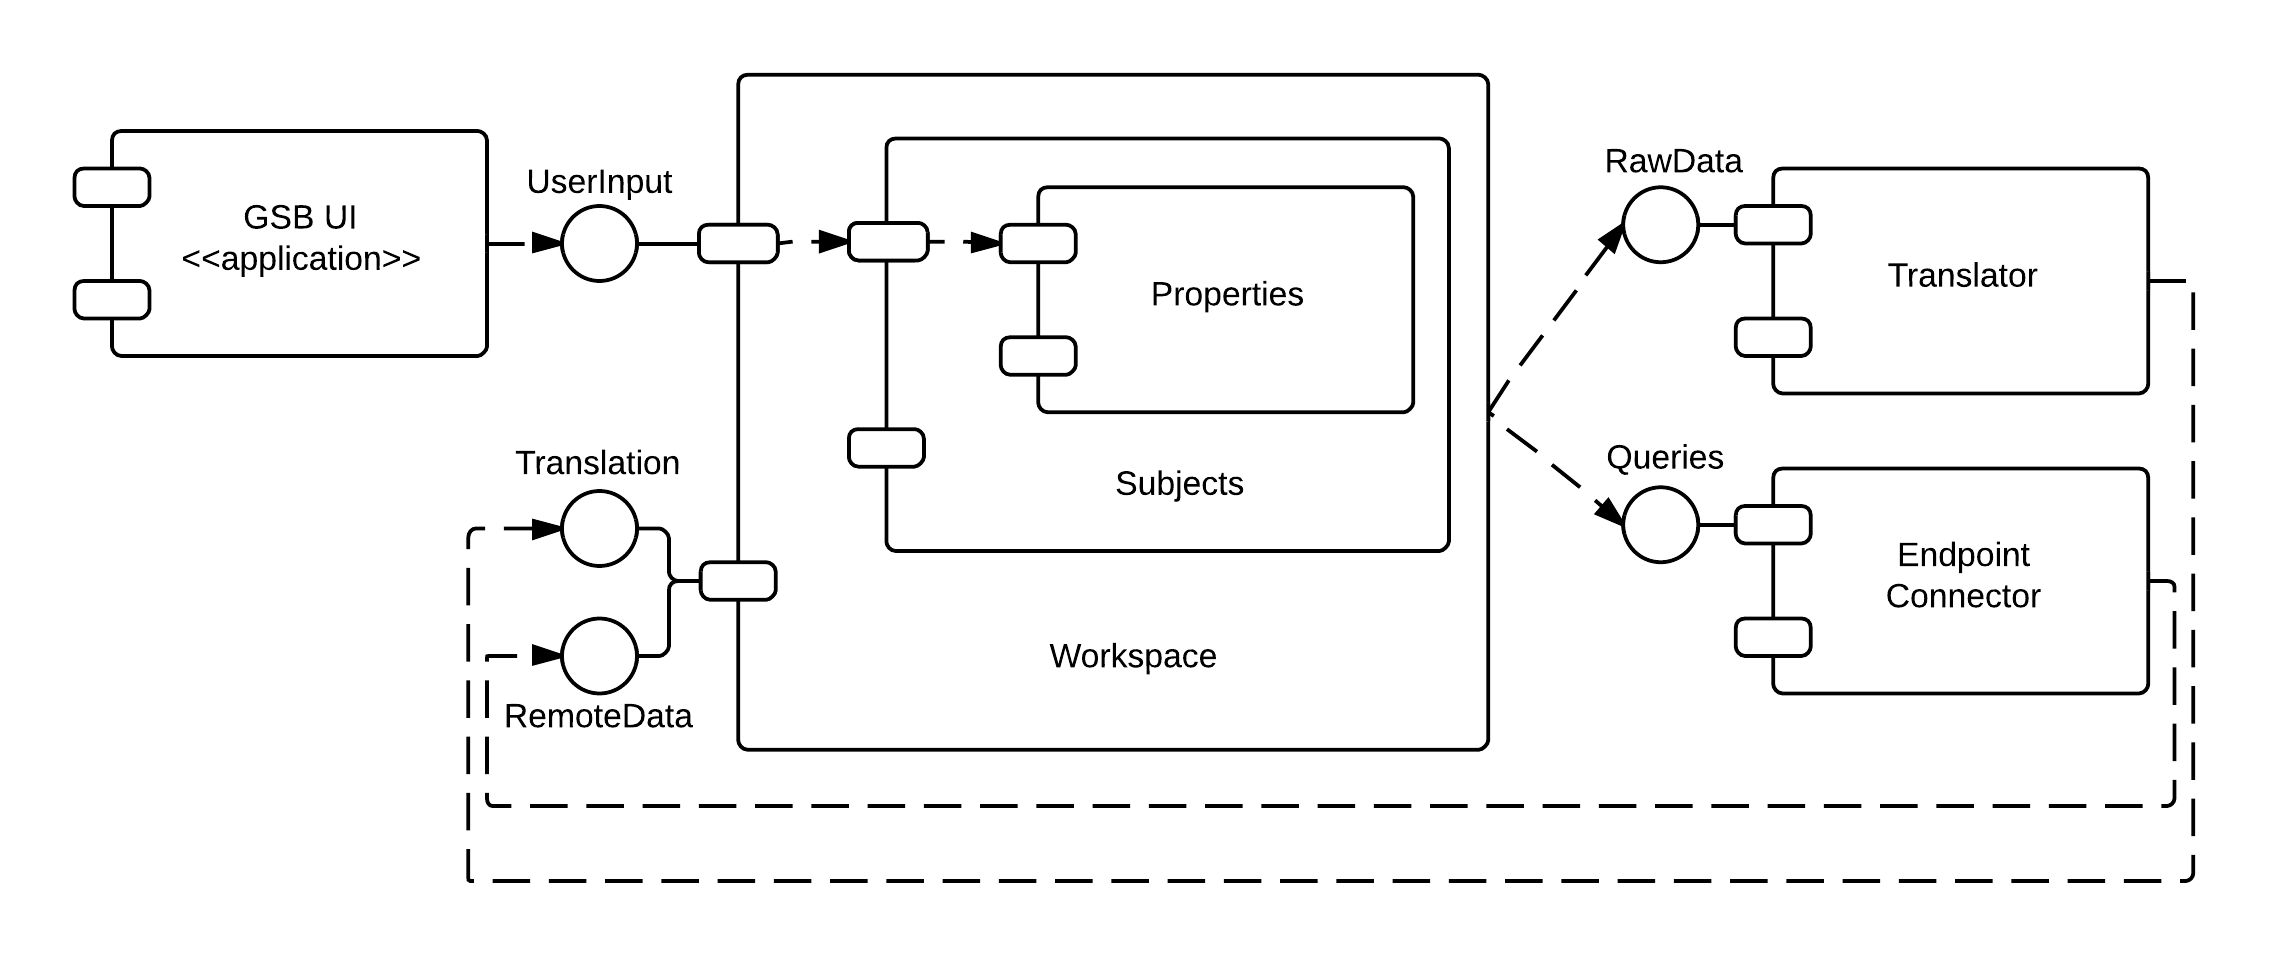
\includegraphics[width=\hsize]{Komponentendiagramm.png}
\caption{Komponentendiagramm des GSB.}
\label{fig02}
\end{figure}
%\end{SCfigure}


Es gibt die Komponente des User Interface (GSB UI), in welcher alle
Eingaben des Benutzers des Tools stattfinden. Diese werden in die
Komponente Workspace weitergeleitet und dort gegebenenfalls an die
Komponenten Subjects und deren Unterkomponente Properties
weitergeleitet. Um dies zu verdeutlichen, hier drei Beispiele:
\begin{enumerate}
\item Der Nutzer setzt eine Übersetzung eines GSBl-Wortes in Gang, dies betrifft die Komponente “Workspace”
\item Der Nutzer ändert den Alias eines Subjekts, dies würde über die Workspace-Komponente zu der Subjects-Komponente weitergereicht werden.
\item Der Nutzer ändert die Sichtbarkeit einer Eigenschaft, dies würde über die Workspace-Komponente zu der Subjects-Komponente zum Ziel, der Properties-Komponente, weitergereicht werden.
\end{enumerate}
Die Workspace-Komponente steht in Verbindung mit der
Translator-Komponente, welche für die Übersetzung der erstellten
Rohdaten zu JSON bzw. SPARQL zuständig ist und die Ergebnisse zurück
zur Workspace-Komponente überträgt.
Ebenso gibt es eine Verbindung zur MockupData-Komponente, welche auf Anfrage der Workspace-Komponente die verfügbaren Subjekte und deren Eigenschaften bereitstellt.


\section{Struktur- und Entwurfsprinzipien einzelner Pakete}

\subsection*{User Interface}

Beim Vorprojekt besteht das Userinterface aus dem Workspace, der die graphisch konstruierte Abfrage beinhaltet, dem Feld in dem nach dem Drücken des "Build Query"-Buttons die Übersetzung der Anfrage in JSON und in SPARQL zu sehen ist. Im Workspace befindet sich der Hinzufüge-Button für Subjekte sowie ein LIST ALL Objekt. Standardmäßig werden zu Beginn zwei Subjekte (Mensch \& Stadt) in den Workspace geladen. Subjekte und Properties sind durch Icons entfernbar sowie in der Abfrage anzeigbar.
Ein Link über dem SPARQL-Result-Feld ermöglicht zusätzlich das Anzeigen des Ergebnisses der übersetzten Anfrage, welches zurückgegeben wird nachdem die Anfrage an einen DBpedia-Endpunkt (Virtuoso) geschickt wurde.

\subsection*{Workspace}

Der Workspace umfasst die Sammlung von Subjekten und den Startpunkt.

\subsection*{Subjects}

Subjects können durch die Icons entfernt (Papierkorb), in der Anfrage aus-/eingeblendet (Auge) und hinzugefügt (Plussymbol) werden.
Subjects sind Instanzen die mit den jeweiligen "externen" Properties Verbindungen untereinander aufbauen und Subject-interne Properties sammeln. Sie bilden somit den grundsätzlichen
Anhaltspunkt für die Übersetzung. (siehe Translator)

\subsection*{Properties}

Properties können durch die Icons entfernt (Papierkorb), in der Anfrage aus-/eingeblendet (Auge) und hinzugefügt (Add-Button beim Subject-Mouseover) werden.
Sie stellen über eine Auswahl im DropDown Menü eines Subjects Verbindungen zwischen Subjects her.

\subsection*{Translator}

Die Translator-Funktion ist im Vorprojekt zweigeteilt. Eine Übersetzung liefert auf Basis der im Workspace zusammengestellten graphischen Anfrage (in GSBL) eine Abfrage im
JSON-Format und eine weitere Übersetzung von JSON in SPARQL wird danach durchgeführt.
Die Translation wird durch Klick auf den Button "Build Query" gestartet und das Ergebnis wird in den unteren Feldern (JSON- \& SPARQL-Resultat) angezeigt.
Algorithmisch betrachtet beginnt die Übersetzung bei dem mit dem Startpunkt verknüpften Subject und übersetzt dann rekursiv alle damit verknüpften Subjects und deren Properties, sodass nicht verknüpfte Subjects ignoriert werden. 

\subsection*{MockupData}

Die Mockup Daten liegen im JSON-Format vor und umfassen die sechs Subjects "Firma", "Universität", "Person", "Stadt", "Land" und "Studiengang" sowie deren Beziehungen untereinander.
Im Vorprojekt ist in der Übersetzung bereits eine Verknüpfung zwischen den Mockup Subejcts und den Subjekten der DBpedia Ontologie realisiert um eine Eindruck der erstellten Abfrage und des Resultats zu ermöglichen. (siehe UI)

\section{Datenmodell}

Die Grundbausteine des RDF-Datenmodells sind Ressourcen, Eigenschaften und Aussagen. Durch diese ist es möglich RDF Ausdrücke syntaxfrei darzustellen.

\subsection*{Ressource}

Eine Ressource wird mit RDF Ausdrücken beschrieben. Folglich muss diese durch eine URI (Universal Resource Identifier) referenzierbar sein und eindeutig von dieser identifiziert werden können.

\subsection*{Eigenschaft}

Eigenschaften sind die Attribute von Ressourcen. Im Datenmodell legen sie die erlaubten Werte, den Typ und die Relation der Ressource zu anderen Ressourcen fest.

\subsection*{Aussage}

Eine Ressource, kombiniert mit ihrer Eigenschaft und den Wert, den die Eigenschaft dieser Ressource hat, nennt man "Aussage". D.h. eine Aussage besteht aus Subjekt-Prädikat-Objekt (Ressource-Eigenschaft-Wert).

\subsection*{Beispiel}

\begin{tabular}{l l}
Aussage  & Der Autor der Ressource ist Herbert Meier \\\midrule
Subjekt  & \url{http://www.example.org/Herbert-Meier} \\
Prädikat & Autor \\
Objekt   & "Herbert Meier"
\end{tabular}

%<Untitled.png>

\section{Testkonzept}

Im Zuge des Vorprojekts wurde auf ein umfassendes Testkonzept
verzichtet.
Da der Fokus auf einem exemplarischen Prototypen liegen
sollte, standen besonders der Aufbau und die Funktionalitäten der GUI
im Vordergrund.
Diese konnten jedoch sehr direkt, ohne spezifische
Tools getestet werden, da Auswirkungen von Änderungen im Code jeweils
unmittelbar und ohne großen manuellen Aufwand überprüfbar waren.
Da die Applikation des Vorprojekts außerdem noch losgelöst von realen Endpoints und Datensätzen arbeitet, sondern mit eigens verfassten Mockup-Daten, waren auch hier keine aufwendigen Tests nötig.
Der JavaScript-Code zuständig für die Übersetzung des JSON-Objekts in
eine SPARQL-Anfrage wurde zunächst separiert von der App geschrieben,
und mithilfe einer simplen HTML-Einbettung regelmäßig auf Fehler
untersucht.
Durch schrittweise Abwechslung von Implementierung und Testläufen wurde dabei sichergestellt, dass jedes Element der GSB-Sprache ordnungsgemäß vom Übersetzer behandelt wird.

Es zeigte sich jedoch, dass mit steigender Komplexität und auch der
zunehmenden Abhängigkeit von externen Daten/Diensten eine
ausgeweitete, protokollierte Teststruktur schnell unabdingbar wird.
So
sollen in der Implementierungsphase des eigentlichen Produkts die
AngularJS-eigenen, sowie externe Testtools wie Protractor eingesetzt
und besonders in den abschließenden Testläufen Protokoll geführt
werden.
Außerdem soll ein besonderes Augenmerk auf Nutzungstests durch
Projekt-fremde User gelegt werden. Dadurch soll Feedback zu den für
den GSB essentiellen Aspekten Benutzbarkeit und Intuitivität gewonnen
werden, von Benutzern die ihrerseits keine Erfahrungen mit SPARQL
haben und sich dadurch mit der Zielgruppe des Projekts decken.

\section{Glossar}

\newcommand{\begriff}[2]{
\paragraph{#1}
#2
}

\begriff{API}
{Application Programming Interface -- Programmierschnittstelle.
Eine API be\hack{-\break}schreibt, wie Software-Komponenten bzw. Programme miteinander interagieren können/sollten. Anders ausgedrückt: eine API ist der Teil eines Softwaresystems, der anderen Programmen zur Verfügung gestellt wird um mit dem Softwaresystem zu interagieren.}

\begriff{DBpedia}
{DBpedia ist eine Datensammlung im RDF Format, deren Datensätze aus der Wikipedia extrahiert wurden. Ziel ist es strukturierte Daten für Webanwendungen zur Verfügung zu stellen.
\cite{dbpedia-wikipedia,dbpedia,dbpedia-datasets}
}

\begriff{Endpoint}
{Ein Endpoint ist eine Schnittstelle zwischen der Datensammlung und der 
Abfragesprache. Nachdem eine Anfrage an den Endpoint gesendet wurde (query)  sendet selbiger die Ergebnisse zurück. Ein Beispiel für einen SPARQL-Endpoint ist der “Virtuoso SPARQL Query Editor”. \cite{dbpedia-sparql}}

\begriff{GSB}
{Graphical SPARQL Builder, der Name des Projekts. \cite{swp14-gsb}}

\begriff{i18n} 
{internationalization and localization -- Anpassung der Software an andere Sprachen und Kulturen ohne Quelltext zu ändern. Sprach- und Kulturspezifika werden über Konfigurationsdateien angepasst.}

\begriff{Ontologie}
{Ontologien sind formalisierte Vokabulare von Begriffen. Diese Vokabulare beziehen sich meist auf eine bestimmte Domäne (Gegenstandsbereich) oder Nutzergruppe. Sie liegen in einer sprachlichen Form vor und umfassen die Begriffe einer Domäne sowie Beziehungen zwischen den Begriffen. \cite{owl,ontologie-wiki,fraunhofer}
}

\begriff{OWL}
{Die Web Ontology Language (OWL, aktuelle Version OWL2) ist eine Beschreibungssprache um Ontologien für das semantische Web zu erstellen und zu publizieren. OWL2-Ontologien können für Informationen verwendet werden, die in RDF geschrieben sind und werden hauptsächlich in Form von RDF-Dokumenten ausgetauscht.
\cite{owl}
}

\begriff{RDF}
{“Resource Description Framework” kurz RDF ist eine Strukturierung von Daten nach
dem Muster Subjekt-Prädikat-Objekt. Alle RDF-Daten werden in diesem Tripel-Format 
gespeichert. RDF gilt als eines der Basis-Elemente des semantischen Webs.
Repräsentationen, also syntaktische Standards, des RDF-Prinzips sind N3 (Notation3), 
Turtle (Terse RDF Triple Language) sowie RDF/XML. Turtle und N3 gelten im Vergleich zu RDF/XML als benutzerfreundlicher. \cite{rdf-primer,rdf-wiki,rdf-xml-wiki}}

\begriff{SPARQL}
{“SPARQL Protocol And RDF Query Language” kurz SPARQL ist eine Abfragesprache für das Datenformat RDF. SPARQL ist graphbasiert und gilt nach dem W3C als Standard für RDF-Abfragen. \cite{w3c-rdf-sparql-query,sparql-wiki}}

\begriff{Triplestore}
{Ein Triplestore ist ein System zur Speicherung, Verwaltung und Bearbeitung einer
 Sammlung von RDF-Tripeln. Ein Triplestore bietet gewöhnlich APIs,
 Rea\-so\-ning-Verfahren sowie Abfragemöglichkeiten. \cite{fraunhofer}}
\newpage
%%%%%%%%%%%%%%%%%%%%%%%%%%%%%%%%%%%%%%%%
\begin{thebibliography}{99}
\bibitem{dbpedia-wikipedia}
  \url{http://de.wikipedia.org/wiki/DBpedia}

\bibitem{dbpedia}
  \url{http://de.dbpedia.org/}

\bibitem{dbpedia-datasets}
  \url{http://wiki.dbpedia.org/Datasets}

\bibitem{dbpedia-sparql}
  \url{http://dbpedia.org/sparql}

\bibitem{swp14-gsb} %5
  \url{http://pcai042.informatik.uni-leipzig.de/~swp14-gsb/}

\bibitem{owl}
  \url{http://www.w3.org/TR/2012/REC-owl2-overview-20121211/}

\bibitem{ontologie-wiki} %10
  \url{http://de.wikipedia.org/wiki/Ontologie}

\bibitem{fraunhofer}
  \url{http://www.iais.fraunhofer.de/fileadmin/user_upload/Abteilungen/OK/PDFs/Alieva_Magisterarbeit.pdf}

\bibitem{rdf-primer}
  \url{http://www.w3.org/TR/rdf-primer/}

\bibitem{rdf-wiki}
  \url{http://de.wikipedia.org/wiki/Resource_Description_Framework}

\bibitem{rdf-xml-wiki}
  \url{https://en.wikipedia.org/wiki/RDF/XML}

\bibitem{w3c-rdf-sparql-query}
  \url{http://www.w3.org/TR/rdf-sparql-query/}

\bibitem{sparql-wiki}
  \url{http://en.wikipedia.org/wiki/SPARQL}

\end{thebibliography}


%%% Local Variables: 
%%% mode: latex
%%% TeX-master: "main"
%%% End: 
